\documentclass[a4paper]{article}
\usepackage{ulem}
\usepackage{setspace}
\usepackage{wrapfig}
\usepackage{bpchem}
\usepackage{color}
\usepackage{subfigure}
\usepackage{float}
\usepackage{titletoc}
\usepackage{indentfirst}
\usepackage{geometry}
\usepackage{amsmath}
\usepackage{amssymb}
\usepackage{graphicx}
\usepackage{enumerate}
\usepackage{url}
\usepackage{caption2}
\usepackage{graphicx}  
\usepackage{epstopdf}
\usepackage{listings}
\lstloadlanguages{[5.2]Mathematica}

\geometry{a4paper,left=2.54cm,right=2.54cm,top=2.54cm,bottom=2.54cm}

\begin {document}
\begin{large}
	\begin{center}
	~\\ ~\\ ~\\ ~\\ ~\\ ~\\ \rule[-1pt]{10.3cm}{0.05em} \\~\\UM-SJTU JOINT INSTITUTE\\~\\Probabilistic Methods in
Engineering\\~\\(VE401)	~\\ \rule[-1pt]{10.3cm}{0.05em} \vspace{7cm} \\Term Project 2
	\end{center}
\end{large}
~\\

\begin{large}
	\begin{center}
	Police Shootings in the United States
	\end{center}
\end{large}
\vspace{5cm}

\begin{tabular}{l l l}
	Name: Feitong Tang&ID: 518370910017&Group 1\\
	Name: Weikai Zhou&ID: 518021911039&Group 1\\
     ~\\
	Date: 30 April 2020
\end{tabular}

\newpage

\section{Abstract}
	Based on David Spiegelhalter and Arthur Barnett's \textit{London murders: a predictable pattern?}, this project analyzes the pattern of occurrence of fatal police shootings in the United States. The project gets its data from the database of the Washington Post and gives an overview of the data. It uses goodness-of-fit test to check whether the occurrence of fatal police shooting in the United States follows a Poisson distribution in the years 2015-2019. It also tests whether the average number of police shootings depends on weekdays. It gives the confidence interval for the parameter $k$ of a Poisson distribution. Based on the data from Jan. 1 to Apr. 15, 2020, it tests whether it follows a Poisson distribution and calculates $\hat{k}_{2020}$. It gives the 95\% prediction intervals for the number of police shootings in 2020 and analyzes how COVID-19 will influence the data for 2020.
\\

\noindent\textbf{Keywords}: Fatal police shooting in the United States, Poisson distribution, goodness-of-fit test, confidence interval, prediction interval.



\newpage

\tableofcontents

\newpage

\section{Introduction}
	\subsection{Background}
	David Spiegelhalter and Arthur Barnett analyzed the pattern of London murders between April 2004 and March 2007, and predicted the number of murders in London during 2008 [1]. Based on their analysis and the data of fatal police shootings in the USA provided by Washington Post [2], we want to analyze the pattern of fatal police shootings in the USA from January 2015, and predict the number of fatal police shootings in 2020.

	\subsection{Objectives}
	\begin{itemize}
	\item Give an overview of the data of fatal police shootings;
	\item Figure out the pattern of fatal police shootings and its dependence on weekday;
	\item Calculate the confidence interval for the parameter of a Poisson distribution;
	\item Predict the numbers of fatal police shootings in 2020;
	\end{itemize}

\section{Data analysis}
	\subsection{Data source}
	The data we use is based on the database of Washington Post. It records every fatal shooting “in which a police officer, in the line of duty, shoots and kills a civilian” since Jan. 1, 2015. This sentence gives the clear definition of “fatal police shooting”, meaning that the database of Washington Post will not document the deaths of those in custody, fatal shootings by officers who are not on duty and non-shooting deaths. Moreover, the Washington Post gets their information mainly from “news accounts, social media postings and police reports”. It also monitors other database like Killed by Police and Fatal Encounters and updates the database regularily with new fatal police shootings and new facts. Therefore, compared with the database of the FBI and the Centers for Disease Control and Prevention, it is more complete [3].

	\subsection{Overview of the data}
	With the help of Mathematica, we can convert the data from Jan. 1, 2015 to Dec. 31, 2019 into a more comprehensible figure, which shows the number of fatal police shootings on each day (Figure 1).
	
	\begin{figure}[H]
	\centering
	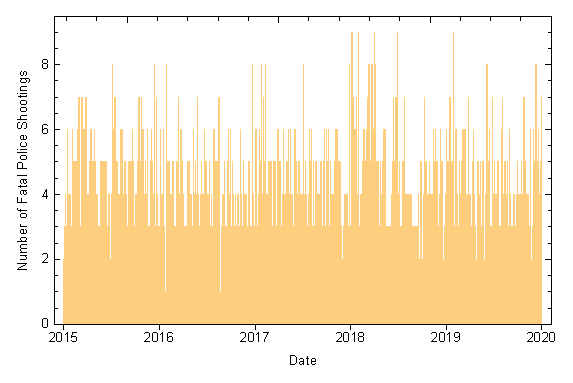
\includegraphics[height=7cm,width=14cm]{Overall(2).eps}
	\caption{Number of fatal police shootings each day from Jan. 1, 2015 to Dec. 31, 2019.}
	\end{figure}

	We notice that there are five days with 9 fatal police shootings recorded and four of them happened in 2018.

\section{Goodness-of-fit test for Poisson distribution}
	In \textit{London murders: a predictable pattern?}, David Spiegelhalter and Arthur Barnett assumed that “if murders happened as random events, the number of murders each day would follow a Poisson distribution” [1]. Similarily, we may assume that the fatal police shootings happened as random events, and the number of fatal police shootings would also follow a Poisson distribution. In order to confirm our assumption, we will test whether the occurrence of fatal police shootings in the USA follows a Poisson distribution or not from 2015 to 2019. From the data, we get the following table (Table 1).

\begin{table}[H]
\centering
\begin{spacing}{1.10}
\begin{tabular}{|c|c|c|c|c|c|c|c|c|c|c|}
\hline
\begin{tabular}[c]{@{}c@{}}Number of fatal police \\ shootings in a day\end{tabular} & 0   & 1   & 2   & 3   & 4   & 5   & 6  & 7  & 8  & 9 \\ \hline
Observed days                                                                    & 139 & 348 & 414 & 382 & 280 & 151 & 66 & 28 & 13 & 5 \\ \hline
\end{tabular}
\end{spacing}
\caption{Observed days with different numbers of fatal police shootings.}
\end{table}

	Let $X$ denotes the number of fatal police shootings in a day, then the maximum-likelihood estimator for $k$ is the sample mean [4], 
\begin{equation}
\begin{split}
\hat{k}=\bar{X}&= \frac{1}{5\cdot365+1} (139\cdot0+348\cdot1+414\cdot2+382\cdot3+ \\  & \quad \   280\cdot4+151\cdot5+66\cdot6+28\cdot7+13\cdot8+5\cdot9) \\
&=2.7043.
\nonumber
\end{split}
\end{equation}

	Then, in order to use the multinomial distribution, we should calculate 
\begin{equation}
\begin{split}
&P[X=0]=\frac{e^{-\hat{k}}{\hat{k}}^0}{0!}=0.0669; \qquad \qquad \qquad P[X=1]=\frac{e^{-\hat{k}}{\hat{k}}^1}{1!}=0.1810;  \\
&P[X=2]=\frac{e^{-\hat{k}}{\hat{k}}^2}{2!}=0.2447; \qquad \qquad \qquad P[X=3]=\frac{e^{-\hat{k}}{\hat{k}}^3}{3!}=0.2206;  \\
&P[X=4]=\frac{e^{-\hat{k}}{\hat{k}}^4}{4!}=0.1491; \qquad \qquad \qquad P[X=5]=\frac{e^{-\hat{k}}{\hat{k}}^5}{5!}=0.0807;  \\
&P[X=6]=\frac{e^{-\hat{k}}{\hat{k}}^6}{6!}=0.0364; \qquad \qquad \qquad P[X=7]=\frac{e^{-\hat{k}}{\hat{k}}^7}{7!}=0.0140;  \\
&P[X=8]=\frac{e^{-\hat{k}}{\hat{k}}^8}{8!}=0.0047;\\
&P[X\ge9]=1-P[X=0]-P[X=1]-\cdots-P[X=8]=0.0019.
\nonumber
\end{split}
\end{equation}

	Therefore, the distribution of $X$ can be expressed as a new distribution with a categorical random variable with parameters $(p_0,\,p_1,\,\cdots,\,p_9)=(0.0669,\, 0.1810,\,\cdots,\,0.0019)$.

	After that, we need to calculate the expected days with $E_i=np_i$, where $i$ is the category and $n$ is the sample size $n=5\cdot365+1=1826$.
\begin{equation}
\begin{split}
&E_0=1826\cdot0.0669=122.19; \qquad \qquad \qquad E_1=1826\cdot0.1810=330.45;  \\
&E_2=1826\cdot0.2447=446.81; \qquad \qquad \qquad E_3=1826\cdot0.2206=402.76;  \\
&E_4=1826\cdot0.1491=272.30; \qquad \qquad \qquad E_5=1826\cdot0.0807=147.27;  \\
&E_6=1826\cdot0.0364=66.38; \qquad \qquad \qquad \,\, \, E_7=1826\cdot0.0140=25.64;  \\
&E_8=1826\cdot0.0047=8.67; \qquad \qquad \qquad\,\, \,\,\, \, E_9=1826\cdot0.0019=3.47.
\nonumber
\end{split}
\end{equation}

	Besides, we should pay attention to the Cochran's Rule, which requires that
\begin{equation}
\begin{split}
&E[X_i]=np_i\ge1\qquad \qquad {\rm for\ all}\ i=1,\,\cdots,\,k,\\
&E[X_i]=np_i\ge5\qquad \qquad {\rm for\ 80\% \ of\ all}\ i=1,\,\cdots,\,k.
\nonumber
\end{split}
\end{equation}

	We find that all of the $E_i$s are greater than 1 and only one out of ten that is smaller than 5, which mean 90\% of the $E_i$s are greater than 5. Therefore, it satisfies the Cochran's Rule, and we can create the following table (Table 2).

\begin{table}[H]
\centering
\begin{spacing}{1.10}
\setlength{\tabcolsep}{1.5mm}{
\begin{tabular}{|c|c|c|c|c|c|c|c|c|c|c|}
\hline
\begin{tabular}[c]{@{}c@{}}Number of fatal police \\ shootings in a day\end{tabular} & 0      & 1      & 2      & 3      & 4      & 5      & 6     & 7     & 8    & 9    \\ \hline
Expected days                                                                        & 122.19 & 330.45 & 446.81 & 402.76 & 272.30 & 147.27 & 66.38 & 25.64 & 8.67 & 3.47 \\ \hline
Obseved days                                                                         & 139    & 348    & 414    & 382    & 280    & 151    & 66    & 28    & 13   & 5    \\ \hline
\end{tabular}}
\end{spacing}
\caption{Expected and observed days with different numbers of fatal police shootings.}
\end{table}

\begin{figure}[H]
\centering
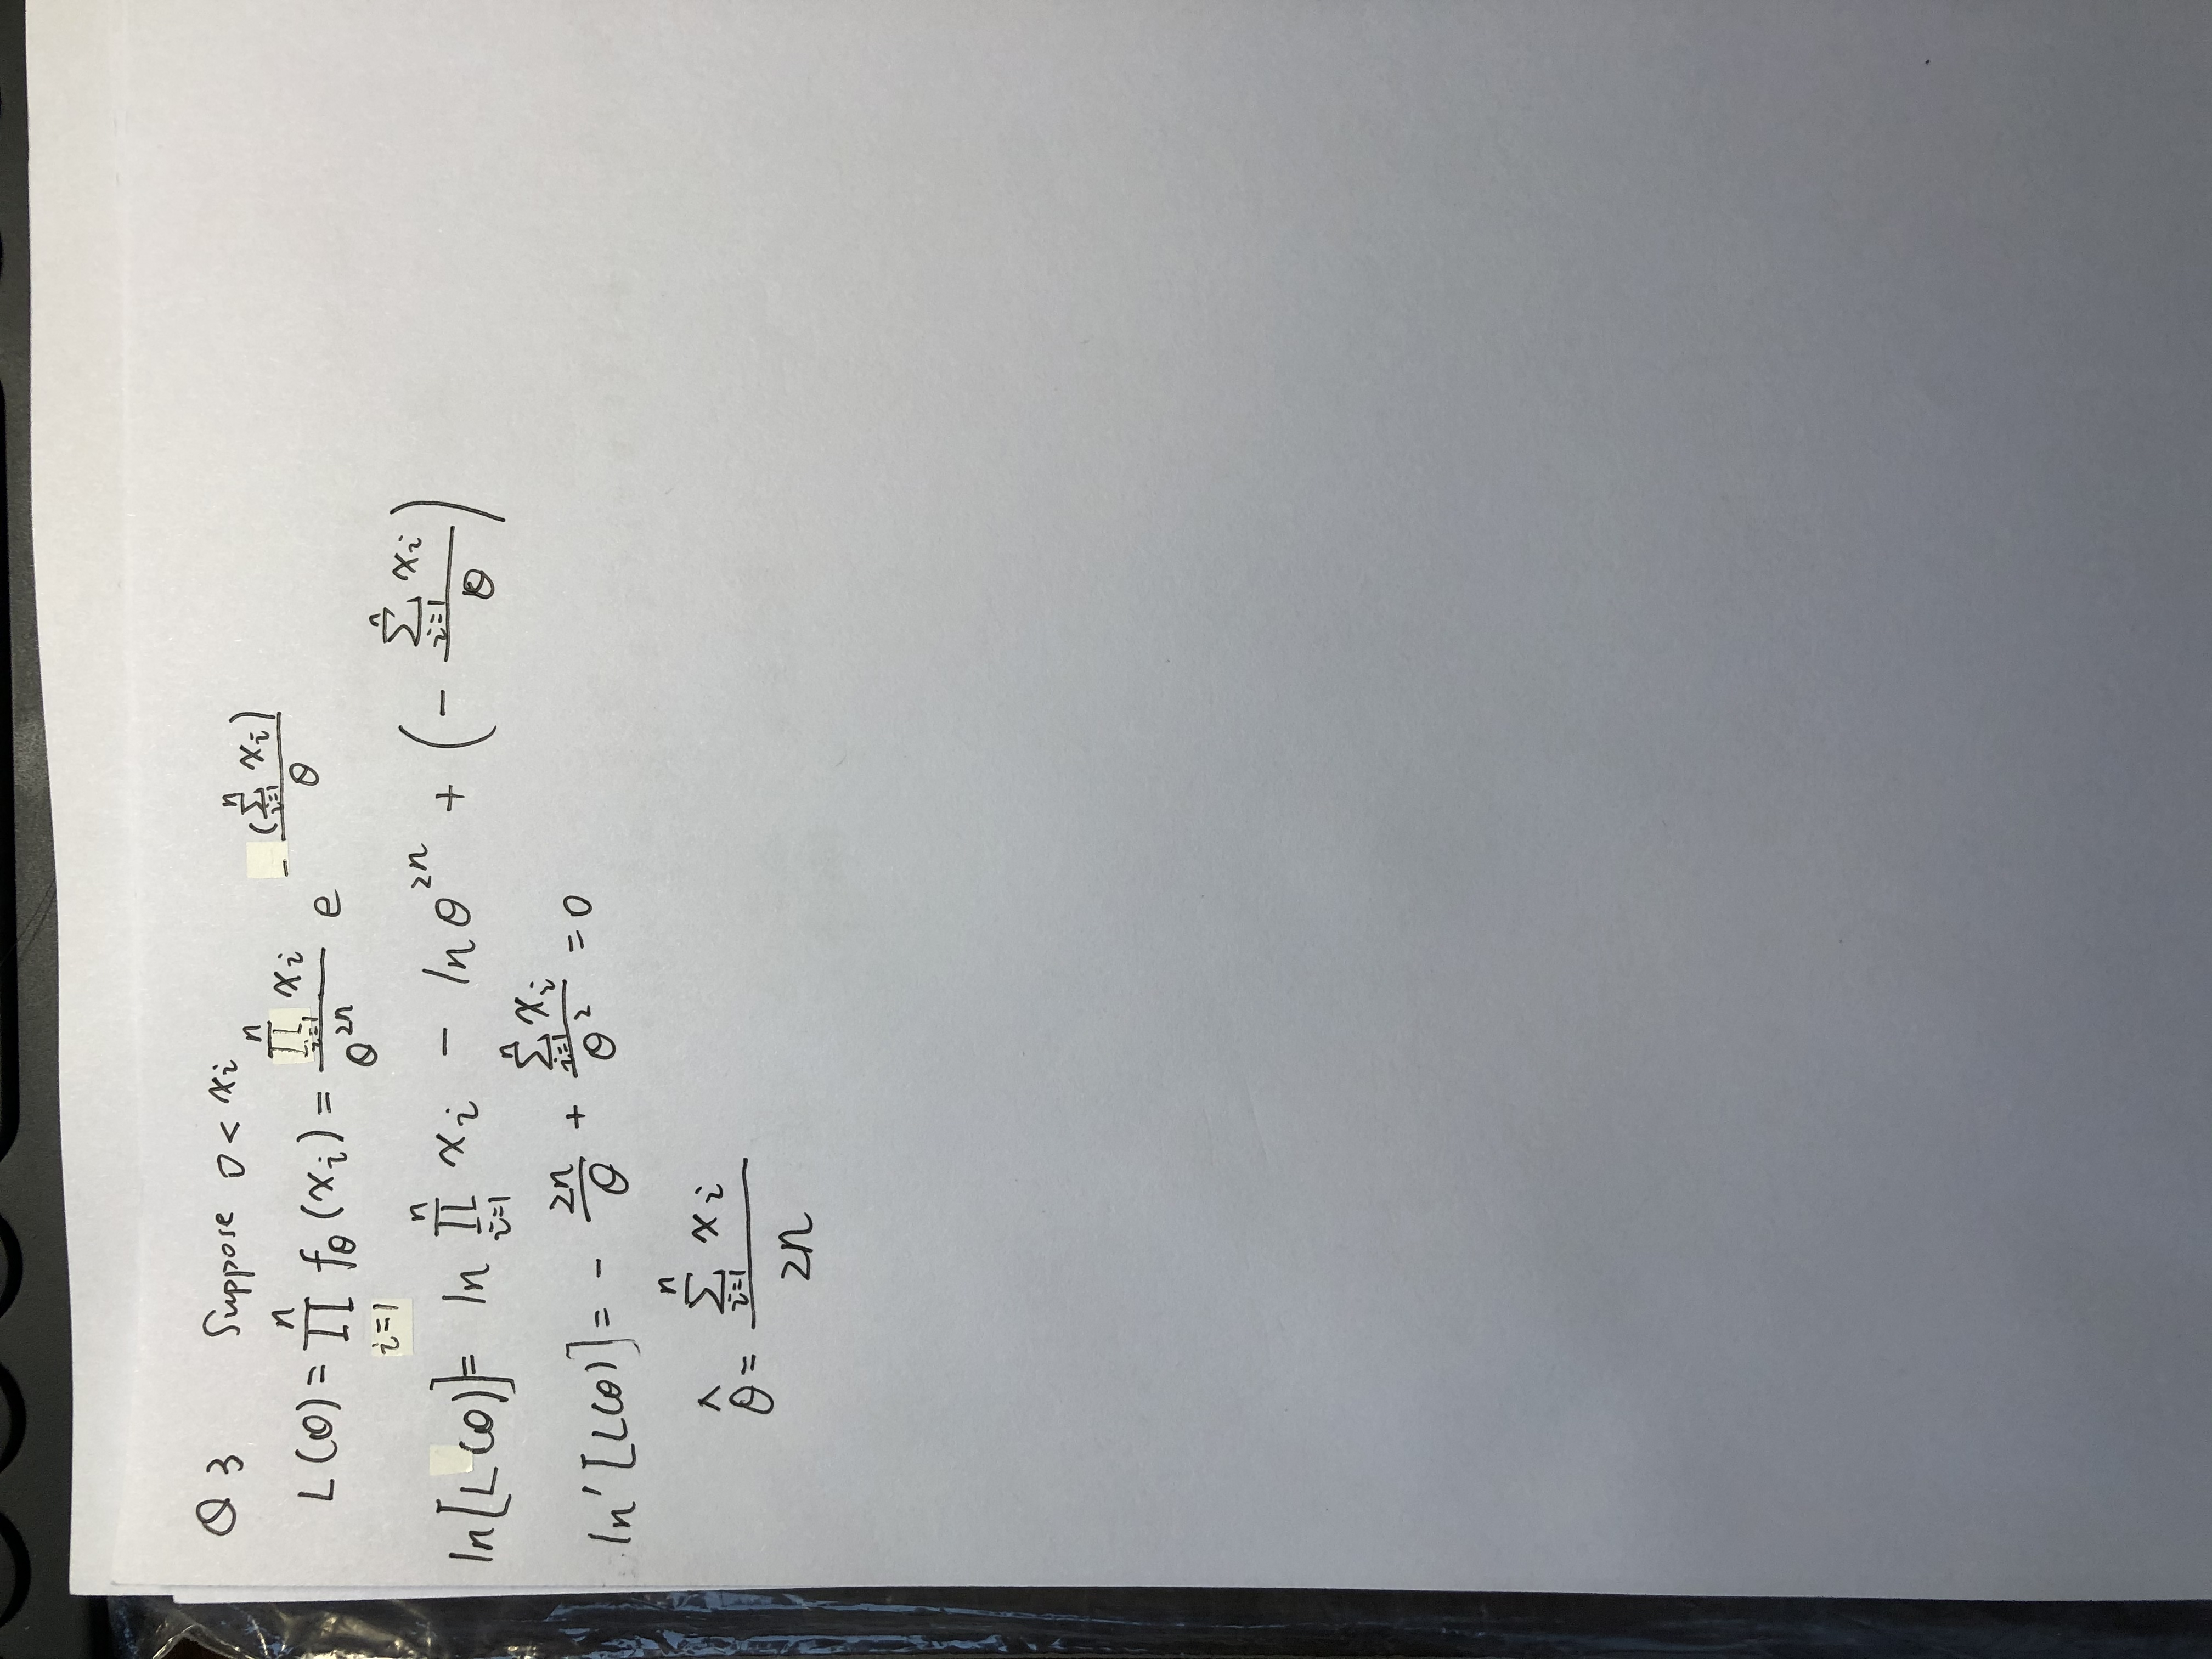
\includegraphics[height=5cm,width=15cm]{3.eps}
\captionsetup{justification=centering}
\caption{Days with different numbers of fatal police shootings: (a) expected; (b) observed.}
\end{figure}

	Then, the hypothesis “$H_0$: the number of fatal police shootings follows a Poisson distribution with parameter $k=2.7043$” is equivalent to “$H_0$: the number of fatal police shootings follows a multinomial distribution with parameters $(0.0669,\, 0.1810,\,\cdots,\,0.0019)$”. Besides, $$X^2=\sum_{i=1}^N\frac{(O_i-E_i)^2}{E_i}$$ follows a chi-squared distribution with $N-1-m=10-1-1=8$ degree of freedom, where $O_i$ is the observed value and $m$ is the number of parameters that we estimate. After we plug in the number, we get $X^2=10.94$. Let $\alpha=0.05$, we have $\chi_{0.05,\,8}^2=15.51\ge10.94$. Therefore, we are unable to reject $H_0$ at the 5\% level of significance. We can calculate the $P$-value as follows $$P=P[X^2|H_0]\le P[\chi_8^2\ge10.94]=1-P[\chi_8^2\le10.94]=1-0.7949=0.2051.$$The $P$-value is quite large, therefore, we cannot reject $H_0$, and we should consider that the number of fatal police shootings during Jan. 1, 2015 and Dec. 31, 2019 follows a Poisson distribution with parameter $k=2.7043$ [5].

\section{Dependence on weekday}
	From the data, we can also create the following figures that shows the number of fatal police shootings on each weekday and month (Figure 3).
\begin{figure}[H]
\centering
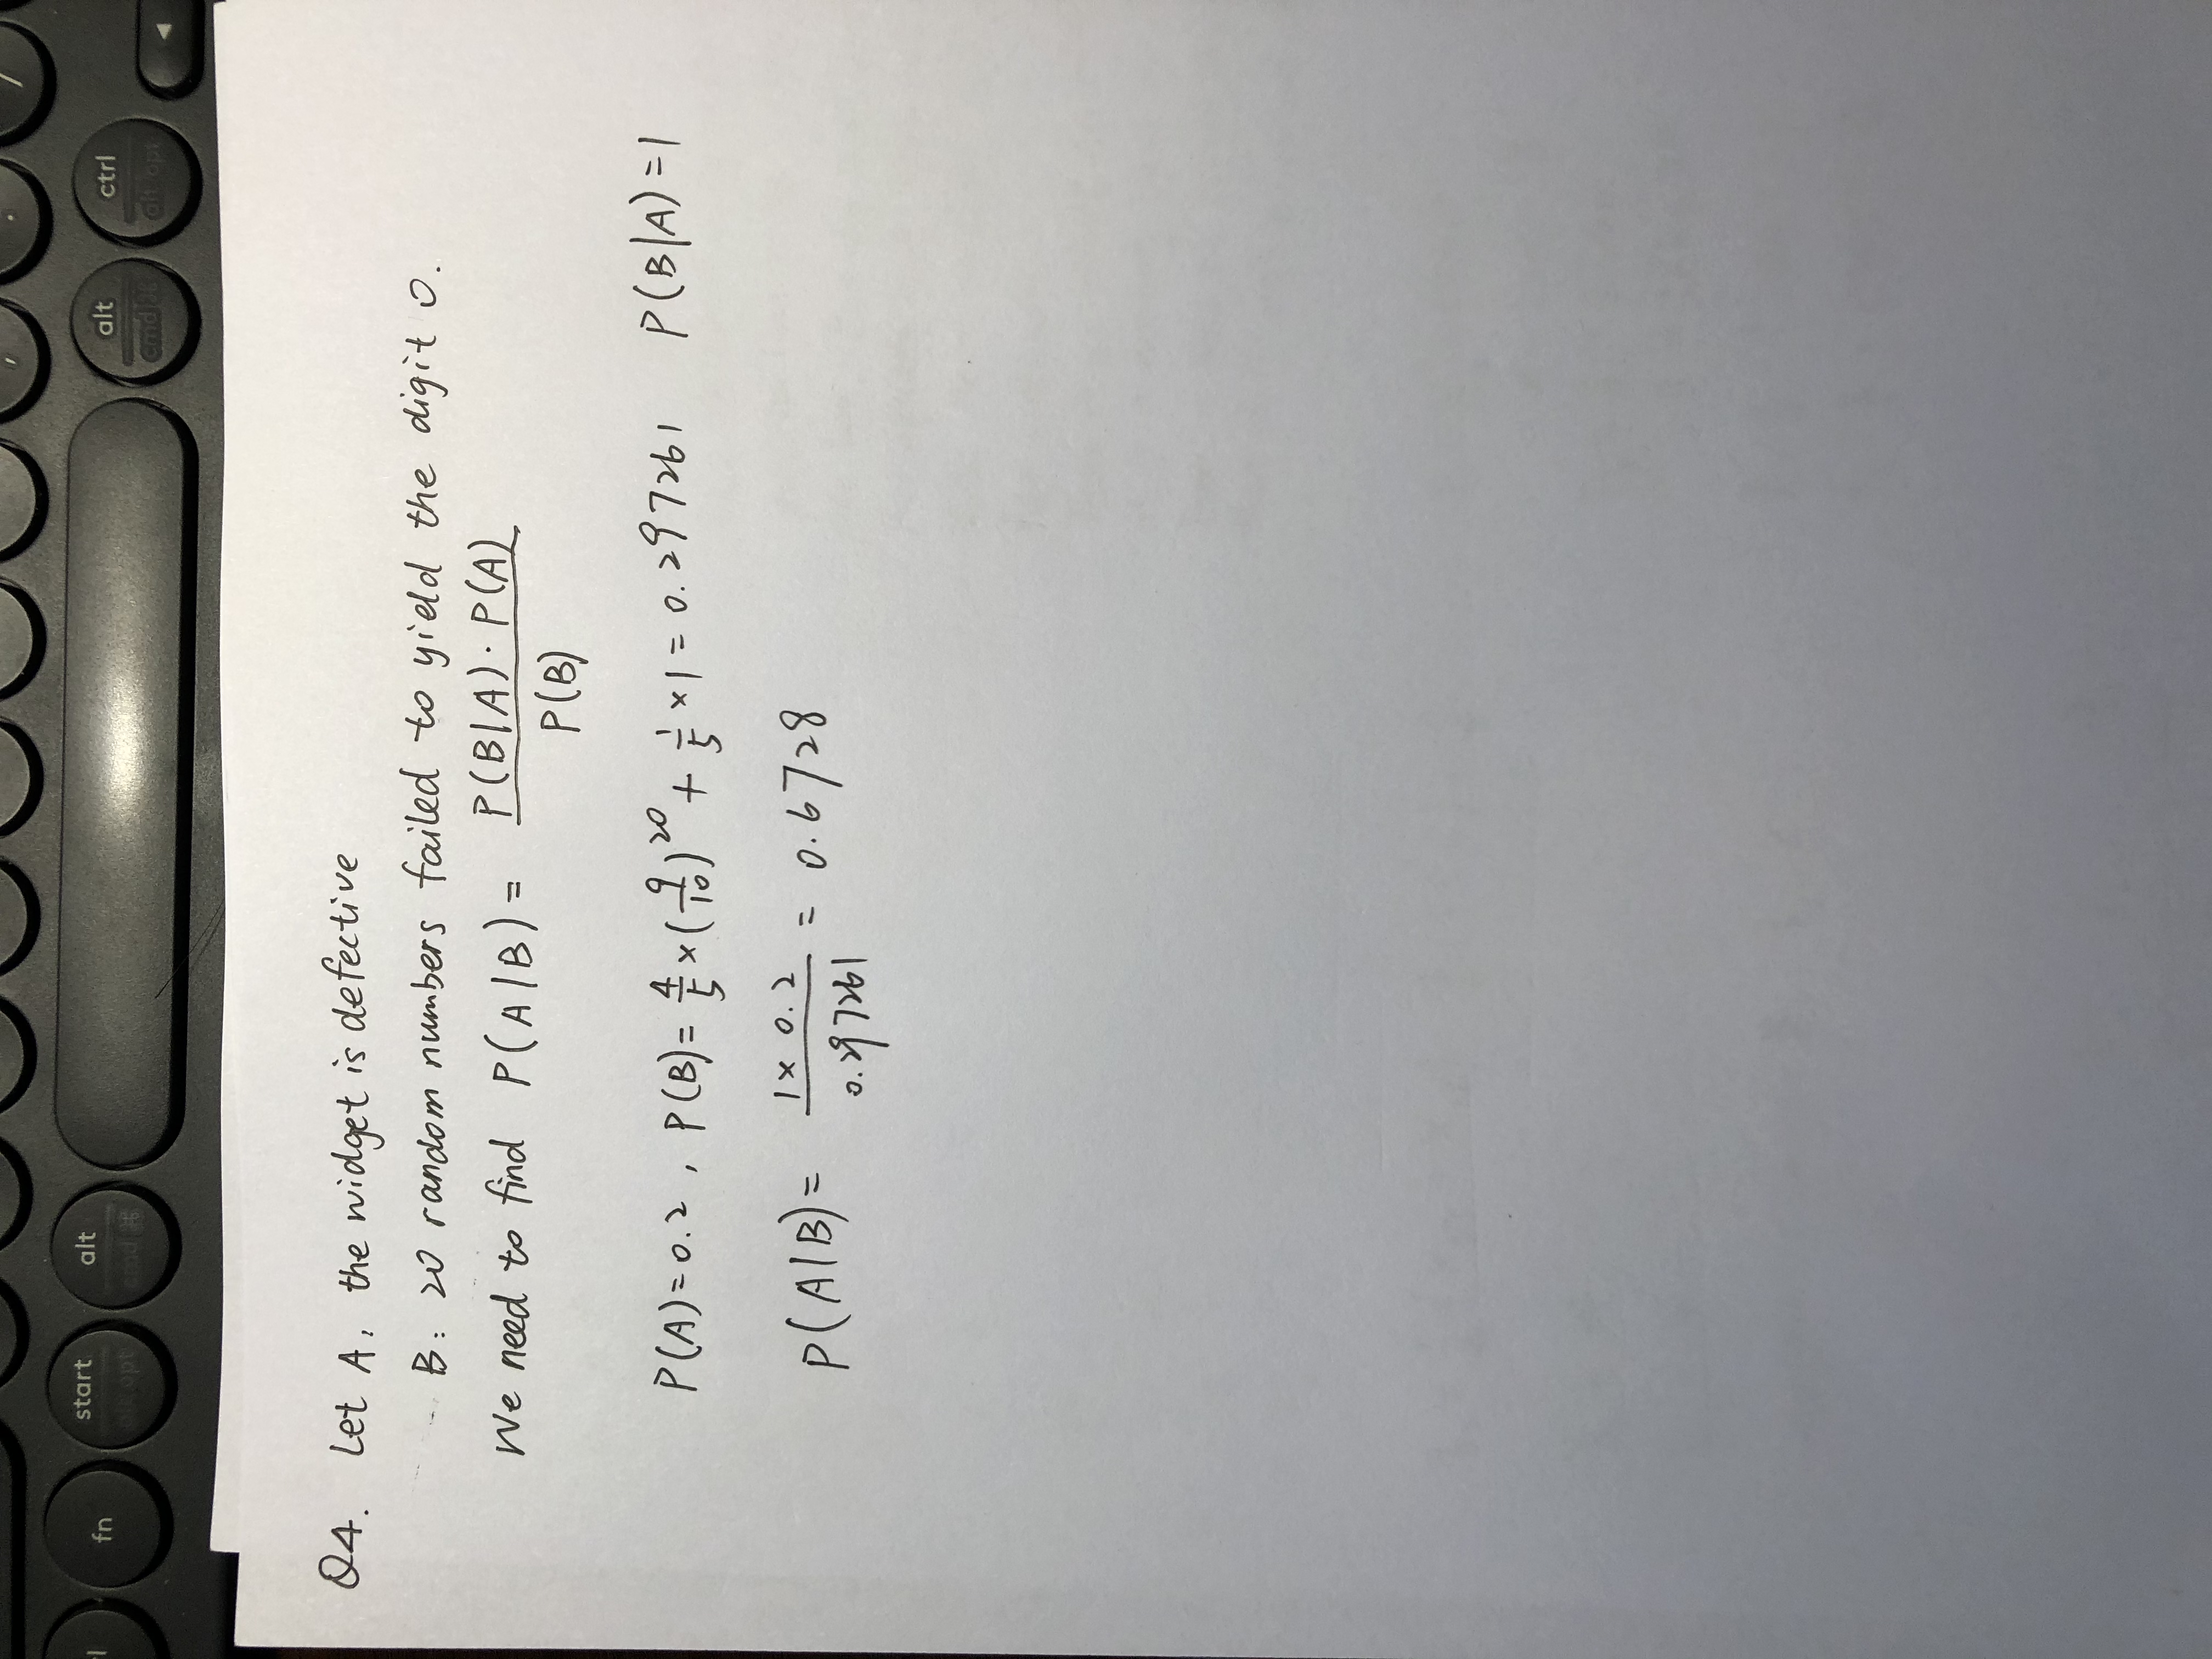
\includegraphics[height=4.5cm,width=13.5cm]{4.eps}
\captionsetup{justification=centering}
\caption{Number of occurrence of police shootings on (a) different weekdays and (b) different months.}
\end{figure}

We want to test whether there is evidence that the average number of police shootings depends on the weekday, then we should set the null hypothesis as “$H_0$: the number of fatal police shootings follows a multinomial distribution with the same parameter $p=\frac{1}{7}$” because there are seven different weekdays. There are 4938 fatal police shootings in total, so we can calculate the expected value on each weekday:
$$E_i=np_i=4938\times\frac{1}{7}=705.43.$$
Then we can get the following table (Table 3).
\begin{table}[H]
\centering
\begin{spacing}{1.10}
\begin{tabular}{|c|c|c|c|c|c|c|c|}
\hline
Weekdays         & Mon.   & Tue.   & Wed.   & Thu.  & Fri.   & Sat.   & Sun.   \\ \hline
Expected numbers & 705.43 & 705.43 & 705.43 & 705.43 & 705.43 & 705.43 & 705.43 \\ \hline
Obseved numbers  & 668    & 742    & 757    & 732    & 692    & 662    & 685    \\ \hline
\end{tabular}
\end{spacing}
\caption{Expected and observed number of fatal police shootings on diferent weekdays.}
\end{table}

We notice that it satisfies the Cochran's Rule because all the $E_i$s are greater than 5. Therfore,
$$X^2=\sum_{i=1}^7\frac{(O_i-E_i)^2}{E_i}=\frac{(668-705.43)^2}{705.43}+\cdots+\frac{(685-705.43)^2}{705.43}=12.17$$ follows a chi-square distribution with $N-1-m=7-1-0=6$ degree of freedom. Let $\alpha=0.05$, we have $\chi_{0.05,\,6}^2=12.59\ge12.17$. Therefore, we fail to reject $H_0$ at the 5\% level of significance, which means we can consider that the occurrence of fatal police shootings is independent on weekdays.




\section{Reference}
[1] D. Spiegelhalter and A. Barnett, “\textit{London murders: a predictable pattern?}” Significance, vol. 6, no. 1, pp. 5–8, 2009. \url{http://onlinelibrary.wiley.com/doi/10.1111/j.1740-9713.2009.00334.x/abstract}.

[2] The Washington Post, “\textit{Data-police-shootings},” GitHub. \url{https://github.com/washingtonpost/data-police-shootings}. Accessed April 19, 2020.

[3] The Washington Post, “\textit{Fata force}.” \url{https://www.washingtonpost.com/graphics/national/police-shootings-2016/}. Accessed April 19, 2020.

[4] H. Hohberger, “\textit{Ve401\_video\_12},” UMJI-SJTU, pp. 18-19, 2020.

[5] H. Hohberger, “\textit{Ve401\_video\_23},” UMJI-SJTU, pp. 9-36, 2020.

\newpage

\section{Appendix}
	\subsection{Code for 3.2 Overview of the data}
\begin{lstlisting}
data := Import["shootingdata.csv"][[2 ;; 4939, 3]]
DateHistogram[data, "Day", 
 Ticks -> {{"2015", "2016", "2017", "2018", "2019", "2020"}, 
   Automatic}, Frame -> True, 
 FrameLabel -> {"Date", "Number of Fatal Police Shootings"}]
\end{lstlisting}
\

	\subsection{Code for 4 Goodness-of-fit test for Poisson distribution}
\begin{lstlisting}
BarChart[{122.19, 330.45, 446.81, 402.76, 272.30, 147.27, 66.38, 
  25.64, 8.67, 3.47}, 
 ChartLabels -> {"0", "1", "2", "3", "4", "5,", "6", "7", "8", 
   "9 or more"}, Frame -> True, 
 FrameLabel -> {"Number of fatal police shootings per day", 
   "Predicted number of occurrences"}, PlotRange -> {0, 450}]

BarChart[{139, 348, 414, 382, 280, 151, 66, 28, 13, 5}, 
 ChartLabels -> {"0", "1", "2", "3", "4", "5,", "6", "7", "8", 
   "9 or more"}, Frame -> True, 
 FrameLabel -> {"Number of fatal police shootings per day", 
   "Actual number of occurrences"}, PlotRange -> {0, 450}, 
 ChartStyle -> Darker[Blue]]
\end{lstlisting}
\

	\subsection{Code for 5 Dependence on weekday}
\begin{lstlisting}
data := Import["shootingdata.csv"][[2 ;; 4939, 3]]
DateHistogram[data, "Day", DateReduction -> "Week", Frame -> True, 
 FrameLabel -> {None, "Number of Fatal Police Shootings"}]
DateHistogram[data, "Month", DateReduction -> "Year", Frame -> True, 
 FrameLabel -> {None, "Number of Fatal Police Shootings"}]
\end{lstlisting}
\end {document}